\documentclass[20pt, a0paper, portrait, blockverticalspace=15mm]{tikzposter}
\usetikzlibrary{positioning}

\title{\parbox{\linewidth}{\centering Spin Motion Perturbation Effect on the EDM Statistic in the Frequency Domain Method}}
\author{A.E. Aksentyev\textsuperscript{1,2,3}, Y.V. Senichev\textsuperscript{3}}
\institute{
  \textsuperscript{1} National Research Nuclear University ``MEPhI,'' Moscow, Russia \\
  \textsuperscript{2} Institut f\"ur Kernphysik, Forschungszentrum J\"ulich, J\"ulich, Germany\\
  \textsuperscript{3} Institute for Nuclear Research of the Russian Academy of Sciences, Moscow, Russia
}


\usetheme{Simple}
\usecolorstyle{Russia}
\colorlet{blocktitlefgcolor}{black}

\usepackage{mathtools}
\usepackage{amsmath}
\usepackage{xparse}
\usepackage{caption}
\captionsetup{font=large}


\let\oldvec\vec
\renewcommand{\vec}{\boldsymbol}
\DeclareDocumentCommand{\bkt}{sm}{\IfBooleanTF{#1}{\left[ #2 \right]}{\left(#2\right)}}
\DeclareDocumentCommand{\ddt}{m}{\frac{\mathrm{d} {#1}}{\mathrm{d} t}}
\DeclareDocumentCommand{\pddx}{mO{t}O{}}{\frac{\partial^{#3} {#1}}{\partial {#2}^{#3}}}
\newcommand{\w}{\omega}
\newcommand{\W}{\Omega}
\newcommand{\avg}[1]{\langle {#1} \rangle}
\newcommand{\nbar}{\bar n}
\newcommand{\ntrn}{n_{turn}}

\begin{document}

\maketitle

\block{INTRODUCTION}{
  The Frequency Domain method of search for the EDM of a particle consists in measuring the combined
  MDM+EDM spin precession frequency in two situations: beam circulating clockwise (direct), and
  counter-clockwise (time-reversed). When these frequencies are added up, the MDM effect cancels, leaving
  only the EDM in the final statistic.\\

  The frequency in question is estimated by fitting a sine function to polarimetry data. However, variation of
  the spin precession angular velocity vector introduces a mismatch between the constant-parameter sinusioidal
  model and measurement data.\\

  Model specification errors are prone to introducing biases into parameter estimates.
  The purpose of this work is to analyze the effect of spin motion perturbation on the EDM statistic.
}

\begin{columns}
  \column{.5}
  \block{PROBLEM STATEMENT}{
    Solution of the T-BMT equation for the
    vertical spin-vector component:
    \begin{equation}\label{eq:master}
      s_y(n_{turn}) = \sqrt{\bkt{\nbar_y\nbar_z}^2 + \nbar_x^2}\cdot\sin\bkt{2\pi\nu_s\cdot\ntrn + \delta}.
    \end{equation}
    Here
    \begin{itemize}
    \item the \emph{invariant spin axis} $\nbar$ defines the orientation of the spin precession angular
      velocity vector;
    \item \emph{spin tune} $\nu_s$ defines the magnitude of the vector.\\
    \end{itemize}

    Significant variation of $\nbar$ and/or $\nu_s$ can lead to model specification error.
  }

  \block{SIMULATION}{
    \begin{tikzfigure}
      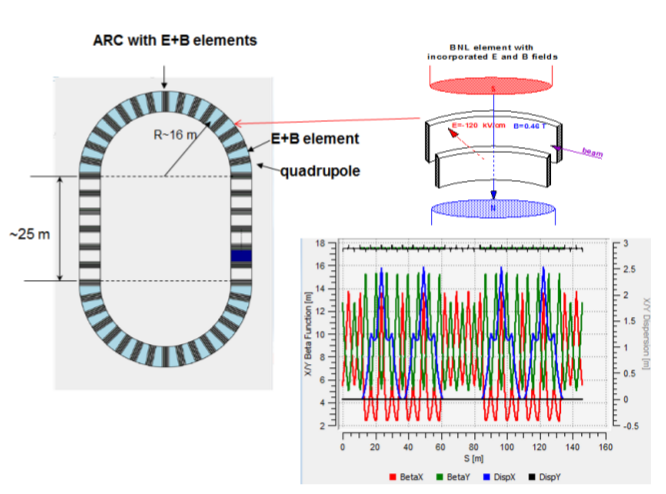
\includegraphics[width=\linewidth]{../img/Lattice/BNL}
    \end{tikzfigure}
    \captionof{figure}{Imperfect Frozen Spin lattice in which sextupole spin decoherence suppression is
      implemented}
    \vspace*{1cm}

    \begin{minipage}[t]{.5\linewidth}
      \textbf{Machine imperfections}
      \begin{itemize}
      \item rotations of E+B spin rotator elements about the optic axis by
        $\alpha \sim N(\mu_i, 3\cdot 10^{-4})$ degrees;;
      \item $\mu_i \in [-1.5\cdot10^{-4}, +2.5\cdot10^{-4}]$ degrees
      \item $\mu_i$ simulates the application of a Spin Wheel.
      \end{itemize}
    \end{minipage}
    \begin{minipage}[t]{.5\linewidth}
      \textbf{Particle}
      \begin{itemize}
      \item 0.3 mm offset from the reference orbit --- vertical plane betatron oscillations;
      \item injection kinetic energy slightly off Frozen Spin;
      \item small $\nbar_x$ value --- increased sensitivity to perturbations.
      \end{itemize}
    \end{minipage}
  }

  \column{.5}
  \block{ANALYSIS}{
    \begin{minipage}[t]{.5\linewidth}
    \textbf{Three data series}
    \begin{itemize}
    \item[TRK] $S_y$ data generated by the COSY INFINITY TR command;
    \item[GEN] $S_y$ data computed from equation~\eqref{eq:master} with $\nbar$, $\nu_s$ the
      TSS command output;
    \item[IDL] $S_y$ as in GEN, but $\nbar = \avg{\nbar(t)}$, $\nu_s = \avg{\nu_s(t)}$.
    \end{itemize}
    \end{minipage}
  }
  \block{CONCLUSIONS}{}
\end{columns}

\end{document}
